\chapter{Methodology}\label{chap:method}

\section{Proposed Solution}

Building on the work of Gordillo et al. \cite{sgame2020}, our solution addresses key limitations in their approach. While SGAME provides a platform for creating educational video games by integrating SCORM-compliant learning objects, it has notable restrictions. Specifically, the game creation process in SGAME is confined to combining pre-existing games with a predefined set of educational questions in various fields. Furthermore, the system’s support for educational content is limited to the Spanish language, which significantly restricts its usability for users from diverse linguistic and cultural backgrounds.

To overcome these limitations, our tool is designed to provide users with greater control over the educational content they can add to their games. Unlike SGAME, which ties games to fixed educational fields, our solution allows the same game template to be adapted for different educational contexts. This approach ensures flexibility, enabling instructors to create games tailored to their specific educational needs and in their preferred language. However, we recognize that certain game templates may naturally align better with specific fields, and such constraints will be accounted for to maintain educational and gameplay coherence.

By addressing these limitations, our tool not only enhances inclusivity and usability but also fosters a more customizable and versatile approach to creating educational games, empowering instructors to provide engaging and context-specific learning experiences.

\section{System Architecture}
Since we are trying to achieve a tool that can be accessed from various devices and platforms, we are using a web-based architecture. The instructor will use a portal to create the game and share it via a link, QR code, or game code with the students. The students will be able to access the game from their devices, and the game will run on any device with a web browser.

We also use a Backend as a Service (BaaS) in the cloud to store the data of the games created, as shown in Figure \ref{fig:architecture}. In our case, we are using Firebase. This allows the data to be stored in the cloud, making the game accessible from anywhere.

The portal is created using Next.js, a React framework, which allows us to build a server-side rendered application. We have developed two game templates: a Space Invaders-like game, which was developed using Unity and hosted on itch.io, and a click-based puzzle game developed using Next.js. More details on these games are provided in the next section.

\begin{figure}
\centering
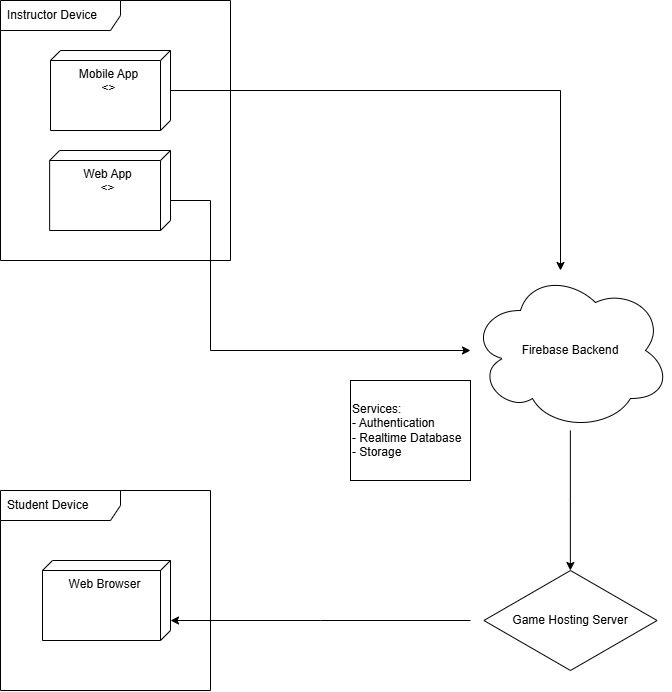
\includegraphics[width=0.8\textwidth]{figures/Deployment_UML.jpg}
\caption{System Architecture}
\label{fig:architecture}
\end{figure}

\section{Instructor Portal}
The instructor portal is a web application that serves to be the tool for generating the game(s), and by generating we mean pushing data to the firebase real-time database, 
and if there is an image like the click-based puzzle game, 
it will upload the image to firebase storage, atleast that was the plan, 
but unfortanly by the time of implementation firebase cahnged their pricing policy and we had to change our approach and use a different storage solution, 
the one we used was Appwrite, which is a similar service to firebase but with a different pricing policy and is open source.
after the data is pushed to the database, the portal will generate a link, a QR code, and a game code that the instructor can share with the students.


\section{Game Templates}
We have developed two game templates: a Space Invaders-like game and a click-based puzzle game. The games are designed to be easily customizable,
allowing the instructor to add their own educational content. The Space Invaders-like game is inspired by the classic arcade game Space Invaders, 
which features fast-paced gameplay where the player must shoot enemies before they reach the bottom of the screen or hit the player with a projectile. In contrast, 
the click-based puzzle game is a more relaxed experience, where the player must solve a puzzle by clicking on the correct answer in the provided image.

\subsection{Space Invaders-like Game}

\subsection{Click-based Puzzle Game}

